\documentclass[9pt,serif,usenames,dvipsnames]{beamer}
\usetheme[progressbar=none]{metropolis}

\useoutertheme{metropolis}
\useinnertheme{metropolis}
\usefonttheme{metropolis}
\usecolortheme{beaver}

% ── Palette colori personalizzata (verde) ────────────────────────────
\definecolor{customgreen}{RGB}{0,128,0}
\definecolor{darkgray}{RGB}{64,64,64}
\definecolor{lightgray}{RGB}{128,128,128}
\definecolor{MSUgreen}{RGB}{0,192,0}

\setbeamercolor{structure}{fg=customgreen}
\setbeamercolor{frametitle}{fg=customgreen}
\setbeamercolor{title}{fg=customgreen}
\setbeamercolor{author}{fg=customgreen}
\setbeamercolor{date}{fg=customgreen}
\setbeamercolor{section in toc}{fg=customgreen}
\setbeamercolor{subsection in toc}{fg=customgreen}
\setbeamercolor{item}{fg=customgreen}
\setbeamercolor{subitem}{fg=customgreen}
\setbeamercolor{subsubitem}{fg=customgreen}
\setbeamercolor{section in head/foot}{fg=customgreen}
\setbeamercolor{subsection in head/foot}{fg=customgreen}
\setbeamercolor{titlelike}{fg=customgreen}
\setbeamercolor{section title}{fg=customgreen}
\setbeamercolor{section name}{fg=customgreen}
\setbeamercolor{separation line}{fg=customgreen}
\setbeamercolor{fine separation line}{fg=customgreen}
\setbeamercolor{progress bar}{fg=customgreen,bg=customgreen!30}
\setbeamercolor{alerted text}{fg=customgreen}
\setbeamercolor{block title alerted}{bg=customgreen,fg=white}
\setbeamercolor{block body alerted}{bg=customgreen!10,fg=black}
\setbeamercolor{block title example}{bg=customgreen!70,fg=white}
\setbeamercolor{block body example}{bg=customgreen!5,fg=black}
\setbeamercolor{block body}{bg=mDarkTeal!5}
\setbeamercolor{block title}{bg=mDarkTeal,fg=black!2}

\setbeamertemplate{footline}[frame number]
\setbeamertemplate{page number in head/foot}[totalframenumber]
\setbeamercolor{background canvas}{bg=white}
\setbeamercovered{transparent=15}
\setbeamersize{text margin left=5mm,text margin right=5mm}
\setbeamertemplate{theorems}[ams style]
\setbeamertemplate{navigation symbols}{}
\setbeamertemplate{frametitle}[default][center]

% ── Pacchetti ─────────────────────────────────────────────────────────────────
\usepackage{amsmath,amssymb}
\usepackage[many]{tcolorbox}
\usepackage{multirow,adjustbox,array}
\usepackage{tikz}
\usepackage{xcolor,xspace}
\usepackage{booktabs}
\usepackage[table]{xcolor}
\usepackage{colortbl}
\usepackage{graphicx}
\usetikzlibrary{arrows,shapes,decorations.pathreplacing,arrows.meta,positioning}

% ── Comandi tabella ───────────────────────────────────────────────────────────
\newcommand\Tstrut{\rule{0pt}{2.9ex}}
\newcommand\Bstrut{\rule[-1.2ex]{0pt}{0pt}}
\newcolumntype{x}[1]{>{\centering\let\newline\\\arraybackslash\hspace{0pt}}p{#1}}

\definecolor{placebg}{HTML}{E1F5EE}
\definecolor{placetxt}{HTML}{085041}
\definecolor{placeacc}{HTML}{1D9E75}
\definecolor{attackbg}{HTML}{E6F1FB}
\definecolor{attacktxt}{HTML}{0C447C}
\definecolor{attackacc}{HTML}{378ADD}
\definecolor{fortifybg}{HTML}{FAEEDA}
\definecolor{fortifytxt}{HTML}{633806}
\definecolor{fortifyacc}{HTML}{BA7517}
\definecolor{ellipsisbg}{HTML}{F5F5F3}
\definecolor{ellipsistxt}{HTML}{888780}
 
\newcolumntype{C}[1]{>{\centering\arraybackslash}p{#1}}


% ── Pseudocodice semplice ─────────────────────────────────────────────────────
\newenvironment{pseudocode}{%
	\begin{tabbing}%
		\hspace{1.4em}\=\hspace{1.4em}\=\hspace{1.4em}\=\kill%
	}{%
	\end{tabbing}%
}
\newcommand{\pckw}[1]{\textbf{#1}}
\newcommand{\pccmt}[1]{\textcolor{gray}{\small\textit{// #1}}}

% ── Titolo ────────────────────────────────────────────────────────────────────
\title[]{%
	{\color{darkgray}\rmfamily\itshape\textbf{Un Framework Intelligente per lo
			Sviluppo di Giocatori e Simulazione del Gioco Risk}}%
}

\author[]{%
	{\color{darkgray}\textsc{\textbf{Autore}}} \hfill
	\url{autore@unife.it}%
}

\titlegraphic{%
	\begin{tikzpicture}[overlay, remember picture]
		\node[at=(current page.south east), anchor=south east,
		xshift=-0.5cm, yshift=0.5cm]{%
			%\includegraphics[width=.18\textwidth]{unife.png}%
		};
	\end{tikzpicture}%
}

\institute[]{%
	Alice Zalambani, Davide Caravita, Giacomo Pampalone, Lorenzo Negrini, Marco Perrotta.
}

\date[2026]{{\color{darkgray}2026}}
\subject{Computer Science}

% =============================================================================
\begin{document}
	
	% ── Copertina ────────────────────────────────────────────────────────────────
	% ── Copertina migliorata ────────────────────────────────────────────────
	\begin{frame}[plain, noframenumbering]
		
		\begin{center}
			\vspace{0.8cm}
			
			% Titolo
			{\usebeamerfont{title}
				\color{customgreen}
				\LARGE\textbf{Un Framework Intelligente per lo Sviluppo}\\[0.2cm]
				\LARGE\textbf{di Giocatori e Simulazione del Gioco Risk}
			}
			
			\vspace{0.8cm}
			
			% Sottolineatura elegante
			\color{customgreen}\rule{0.6\textwidth}{0.5pt}
			
			\vspace{1cm}
			
			% Autori
			{\color{darkgray}\large
				\textsc{Alice Zalambani},
				\textsc{Davide Caravita},
				\textsc{Giacomo Pampalone},\\
				\textsc{Lorenzo Negrini},
				\textsc{Marco Perrotta}
			}
			
			\vspace{0.9cm}
			\vspace{1.2cm}
			
			% Università
			{\color{darkgray}\normalsize
				Department of Mathematics and Computer Science\\
				University of Ferrara
			}
			
			\vfill
			
			% Anno
			{\color{lightgray}2026}
			
		\end{center}
		
		% Logo in basso a destra (più discreto)
		\begin{tikzpicture}[overlay, remember picture]
			\node[at=(current page.south east), anchor=south east,
			xshift=-0.5cm, yshift=0.5cm]{%
				%\includegraphics[width=.14\textwidth]{unife.png}%
			};
		\end{tikzpicture}
		
	\end{frame}
	
	% ── Indice ────────────────────────────────────────────────────────────────────
	\begin{frame}
		\frametitle{Outline}
		\setbeamertemplate{itemize item}[ball]
		\setbeamercolor{itemize item}{fg=structure}
		\begin{center}
			\large
			\begin{itemize}
				\setlength{\itemsep}{0.6em}
				\item<1-> Introduzione \& Motivazione
				\item<2-> Modellazione del Gioco
				\item<3-> Bot dalla Letteratura
				\item<4-> Architettura per Giocatori Intelligenti
				\item<5-> Risultati
				\item<6-> Conclusioni
			\end{itemize}
		\end{center}
	\end{frame}
	
	% =============================================================================
	\section{Introduzione \& Motivazione}
	
	\begin{frame}{\centering Introduzione \& Motivazione}
		\textbf{Il contesto:}
		\begin{itemize}
			\item \alert{Risk} è un gioco da tavolo strategico classico: territorio,
			risorse, alleanze e fortuna si intrecciano in modo non banale.
			\item È un ambiente d'interesse per studiare \alert{agenti artificiali} in giochi
			competitivi.
			\item La complessità del dominio lo rende un \alert{benchmark impegnativo}
			per metodi di apprendimento automatico.
		\end{itemize}
		
		\vspace{0.1cm}
		\textbf{Obiettivi:}
		\begin{itemize}
			\item Si vuole creare un framework \alert{aperto, modulare e Python-nativo}
			per la simulazione di Risk e lo sviluppo di agenti.
			\item Si è implementato una suite di bot basati su lavori noti in letteratura;
			\\ tali strategie, \alert{hand-coded}, offrono un punto di riferimento, \alert{ma}
			non apprendono né si adattano, si vogliono superare tali limiti.
		\end{itemize}
		
		
	\end{frame}
	
	% =============================================================================
	\section{Modellazione del Gioco}
	
	\begin{frame}{\centering Modellazione del Gioco , Struttura}
		\begin{columns}[T]
			\begin{column}{0.50\textwidth}
				\begin{block}{Entità principali}
					\small
					\begin{itemize}
						\item \textbf{Map}: grafo di \texttt{Country} e \texttt{Continent};
						gestisce ownership, rinforzi e connettività.
						\item \textbf{GameState}: fase corrente (\textsc{place}/\textsc{attack}/
						\textsc{fortify}), giocatore corrente, leaderboard.
						\item \textbf{Game}: orchestratore di turni; inizializza lo stato,
						interpella i \texttt{player} \\ e aggiorna il visualizzatore.
						\item \textbf{Action}: gerarchia astratta con
						\texttt{PlaceArmyAction}, \texttt{AttackAction},
						\texttt{FortifyAction}.
					\end{itemize}
				\end{block}
			\end{column}
			\begin{column}{0.46\textwidth}
				\begin{center}
					\begin{tikzpicture}[scale=0.82,
						box/.style={rectangle,draw,rounded corners,fill=mDarkTeal!15,
							minimum width=2.6cm,minimum height=0.65cm,font=\small},
						arr/.style={-Stealth,thick,customgreen}]
						\node[box] (game)  at (0,3.7)    {\texttt{Game}};
						\node[box] (gs)    at (0,2.3)    {\texttt{GameState}};
						\node[box] (map)   at (-1.5,1) {\texttt{Map}};
						\node[box] (cont)  at (-1.5,-0.25) {\texttt{Continent}};
						\node[box] (coun)  at (-1.5,-1.5){\texttt{Country}};
						\node[box] (act)   at (2.03,-1.5)  {\texttt{Action}};
						\node[box] (play)  at (2,1)  {\texttt{Player}};
						
						\draw[arr] (game)  -- (gs);
						\draw[arr] (gs)    -- (map);
						\draw[arr] (gs)    -- (play);
						\draw[arr] (map)   -- (cont);
						\draw[arr] (cont)  -- (coun);
						\draw[arr] (play)  -- (act);
						\draw[arr] (act)   -- (coun);
					\end{tikzpicture}
				\end{center}
			\end{column}
		\end{columns}
	\end{frame}
	
	\begin{frame}{\centering Modellazione del Gioco: Turno}
		
		\begin{columns}[T]
			\begin{column}{0.50\textwidth}
				\begin{tcolorbox}[
					enhanced,
					colback=gray!4,
					colframe=customgreen!70,
					boxrule=0.5pt,
					fonttitle=\bfseries\small,
					title={Struttura di un turno}]
					\footnotesize
					\begin{pseudocode}
						\pckw{for each} alive player \pckw{do} \\
						\> set phase $\leftarrow$ \textsc{place} \\
						\> player.turn\_setup() \\[2pt]
						\> \pckw{loop} \\
						\>\> action $\leftarrow$ player.choose\_action() \\
						\>\> \pckw{if} action = $false$ \pckw{then} \\
						\>\>\> advance phase \\
						\>\>\> \pckw{if} phase wraps \pckw{then break} \\
						\>\> \pckw{else} \\
						\>\>\> action.execute() \\
						\> \pckw{end loop} \\
						\pckw{end for}
					\end{pseudocode}
				\end{tcolorbox}
			\end{column}
			
			\begin{column}{0.46\textwidth}
				\vspace{0.1cm}
				\begin{block}{Fasi del turno}
					\small
					\begin{enumerate}
						\item \textbf{Place Army}: il giocatore piazza \\le truppe di rinforzo
						calcolate dalla mappa (bonus continenti + $\lfloor n/3 \rfloor$).
						\item \textbf{Attack}: attacchi illimitati con lancio di dadi classico
						di Risk (max 3 attaccanti vs max 3 difensori).
						\item \textbf{Fortify}: un solo spostamento tra paesi connessi
						per alleanza.
					\end{enumerate}
				\end{block}
				\vspace{0.2cm}
				\begin{block}{Condizione di fine gioco}
					\small
					La partita termina quando \alert{un solo giocatore} sopravvive oppure
					al raggiungimento di un \alert{numero massimo di turni}.
				\end{block}
			\end{column}
		\end{columns}
	\end{frame}
	
	% =============================================================================
	\section{Bot dalla Letteratura}
	
	\section{Angry}
	% ,,,- Angry ,,,,,,,,,,,,,,,,,,,,--
	\begin{frame}{\centering Bot: \texttt{Angry}, Strategia Aggressiva}
		\begin{columns}[T]
			\begin{column}{0.50\textwidth}
				\begin{block}{Strategia}<1->
					\small
					Massimizza la \alert{pressione sui territori nemici}.
					Ogni azione è orientata ad attaccare il più possibile.
				\end{block}
				\begin{block}{Place}<2->
					\small
					Piazza \alert{tutti} i rinforzi nel paese che possiede il
					maggior numero di vicini nemici.
				\end{block}
				\begin{block}{Attack}<3->
					\small
					Ogni paese attacca il vicino nemico \alert{più debole} se ha
					più armate del difensore. Dopo la conquista, \emph{tutte} le
					truppe vengono spostate nel paese con il maggior numero di
					vicini nemici.
				\end{block}
				\begin{block}{Fortify}<4->
					\small
					Cede \emph{tutte} le proprie armate al vicino alleato che ha
					\alert{più nemici}, svuotando i paesi meno esposti.
				\end{block}
			\end{column}
			\begin{column}{0.46\textwidth}
				\begin{center}
					
						\begin{tikzpicture}[scale=0.9,
							own/.style={circle,draw,fill=mDarkTeal!30,minimum size=8mm,font=\tiny},
							enemy/.style={circle,draw,fill=red!30,minimum size=8mm,font=\tiny},
							arr/.style={-Stealth,thick,customgreen}]
							\node[own]   (a) at (0,0)    {$A_2$};
							\node[enemy] (e1) at (2,0.8) {$E_1$};
							\node[enemy] (e2) at (2,-0.8){$E_2$};
							\node[own]   (b) at (-2,0)   {$A_1$};
							\draw[-] (a) -- (e1);
							\draw[arr,dashed,red!70] (a) -- (e2) node[midway,above=2pt,font=\tiny]{attack};
							\draw[arr,dashed,blue!60] (b) -- (a) node[midway,above,font=\tiny]{fortify};
							\node[font=\tiny,text=mDarkTeal] at (0,-1.6)
							{\textcolor{mDarkTeal}{$\bullet$ owned} \quad
								\textcolor{red!70}{$\bullet$ enemy}};
						\end{tikzpicture}
					
				\end{center}
				\vspace{0.3cm}
				\begin{alertblock}{Caratteristica chiave}<6->
					\small
					\alert{Nessuna difesa passiva}: ogni risorsa è concentrata
					nel punto di massima pressione offensiva.
				\end{alertblock}
			\end{column}
		\end{columns}
	\end{frame}

	\section{Stinky}

	% ,,,- Stinky ,,,,,,,,,,,,,,,,,,,,
	\begin{frame}{\centering Bot: \texttt{Stinky}, Strategia Opportunista}
		\begin{columns}[T]
			\begin{column}{0.50\textwidth}
				\begin{block}{Strategia}<1->
					\small
					Usa la \alert{casualità} per il placement; attacca solo
					quando possiede un vantaggio numerico di $\times 1.5$.
				\end{block}
				\vspace{0.1cm}
				\begin{block}{Place}<2->
					\small
					Piazza \alert{tutte} le armate in un paese scelto
					\emph{casualmente}, purché abbia almeno un vicino nemico.
				\end{block}
				\vspace{0.1cm}
				\begin{block}{Attack}<3->
					\small
					Attacca il vicino nemico più debole solo se possiede
					$\mathbf{1.5\times}$ le sue truppe. Dopo la conquista,
					sposta \emph{tutte} le armate nel paese che ha il vicino
					nemico più debole.
				\end{block}
				\vspace{0.1cm}
				\begin{block}{Fortify}<4->
					\small
					\alert{Nessuna fortification}: il bot ignora completamente
					questa fase.
				\end{block}
			\end{column}
			\begin{column}{0.46\textwidth}
				\vspace{0.3cm}
				\onslide <5->{
					\begin{tcolorbox}[
						enhanced,
						colback=yellow!15,
						colframe=yellow!60!orange,
						boxrule=0.5pt,
						fonttitle=\bfseries\small,
						title={Condizione di attacco}]
						\footnotesize
						\[
						\text{attack if} \quad
						\frac{A_{\text{own}}}{A_{\text{enemy}}} \ge 1.5
						\]
					\end{tcolorbox}
				}
				\vspace{0.3cm}
				\begin{alertblock}{Caratteristica chiave}<6->
					\small
					Placement \alert{completamente casuale} ma attacco
					condizionato da una soglia di superiorità fissa.
					Nessuna gestione delle riserve.
				\end{alertblock}
			\end{column}
		\end{columns}
	\end{frame}

	
	\section{Communist}
	% ,,,- Communist ,,,,,,,,,,,,,,,,,,,
	\begin{frame}{\centering Bot: \texttt{Communist}, Strategia Egualitaria}
		\begin{columns}[T]
			\begin{column}{0.50\textwidth}
				\begin{block}{Strategia}<1->
					\small
					\alert{Tutti i paesi sono uguali.} Il bot distribuisce risorse
					uniformemente invece di concentrarle sul fronte.
				\end{block}
				\vspace{0.24cm}
				\begin{block}{Place}<2->
					\small
					Piazza \alert{1 armata alla volta} nel paese posseduto più
					debole (minor numero di truppe), iterando finché non ha
					esaurito i rinforzi disponibili.
				\end{block}
				\vspace{0.24cm}
				\begin{block}{Attack}<3->
					\small
					Attacca il nemico vicino più debole se ha \alert{parità o
						superiorità numerica}. Dopo la conquista le truppe vengono
					distribuite in modo che il paese di origine e quello
					conquistato abbiano lo stesso numero di armate.
				\end{block}
			\end{column}
			\begin{column}{0.46\textwidth}
				\begin{block}{Fortify}<4->
					\small
					\alert{Equalizzazione globale}: l'obiettivo è che ogni paese
					abbia tante armate quanti i propri vicini alleati. Gli
					spostamenti bilanciano i paesi al di sopra e al di sotto
					di questa media.
				\end{block}
				\onslide <5-> {
					\begin{tcolorbox}[
						enhanced,
						colback=red!8,
						colframe=red!50,
						boxrule=0.5pt,
						fonttitle=\bfseries\small,
						title={Fortify: equalizzazione}]
						\footnotesize
						\[
						\text{goal: } A_i = A_{\text{friendly\_neighbors}(i)}
						\]
						\[
						\Delta = \left\lfloor
						\frac{A_{\text{rich}} - A_{\text{poor}}}{2}
						\right\rfloor
						\text{ truppe spostate}
						\]
					\end{tcolorbox}
				}
				\begin{alertblock}{Caratteristica chiave}<6->
					\small
					\alert{Non attacca altri Communist} se esistono avversari di
					altro tipo , emulando una coalizione implicita.
				\end{alertblock}
			\end{column}
		\end{columns}
	\end{frame}
	
	\section{Cluster}
	% ,,,- Cluster ,,,,,,,,,,,,,,,,,,,--
	\begin{frame}{\centering Bot: \texttt{Cluster}, Strategia di Confine}
		\begin{columns}[T]
			\begin{column}{0.50\textwidth}
				\begin{block}{Strategia}<1->
					\small
					Consolida il controllo sul \alert{miglior cluster continentale}:
					un sottoinsieme connesso di paesi nello stesso continente,
					valutato in base alla dimensione del continente maggiore
					posseduto.
				\end{block}
				\vspace{0.42cm}
				\begin{block}{Place}<2->
					\small
					Distribuisce i rinforzi \alert{lungo il confine del cluster
						migliore}, rinforzando prima il paese di frontiera più debole.
				\end{block}
				\vspace{0.42cm}
				\begin{block}{Attack}<3->
					\small
					I paesi di confine del cluster attaccano i vicini nemici con
					\alert{meno armate}. Dopo la conquista, le truppe vengono
					spostate verso il paese con il vicino nemico più debole.
				\end{block}
				\vspace{0.42cm}
			\end{column}
			\begin{column}{0.46\textwidth}
				\begin{block}{Fortify}<4->
					\small
					Le armate vengono spostate \alert{verso l'esterno del cluster},
					in direzione dei confini, bilanciando le frontiere.
				\end{block}
				\begin{center}
					
						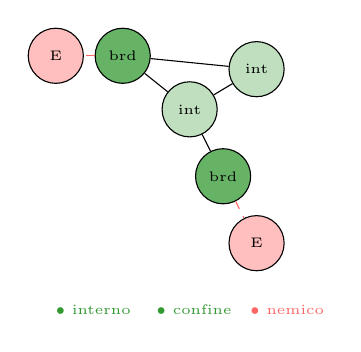
\begin{tikzpicture}[scale=0.85,
							intr/.style={circle,draw,fill=customgreen!25,minimum size=7mm,font=\tiny},
							bord/.style={circle,draw,fill=customgreen!60,minimum size=7mm,font=\tiny},
							enemy/.style={circle,draw,fill=red!25,minimum size=7mm,font=\tiny}]
							
							\node[intr]  (i1) at (0,0)     {int};
							\node[intr]  (i2) at (1,0.6)   {int};
							\node[bord]  (b1) at (-1,0.8)  {brd};
							\node[bord]  (b2) at (0.5,-1)  {brd};
							\node[enemy] (e1) at (-2,0.8)  {E};
							\node[enemy] (e2) at (1,-2)    {E};
							
							\draw (i1)--(i2); \draw (i1)--(b1); \draw (i1)--(b2);
							\draw (i2)--(b1);
							\draw[dashed,red!60] (b1)--(e1);
							\draw[dashed,red!60] (b2)--(e2);
							\node[font=\tiny] at (0,-3){
								\textcolor{customgreen!80}{$\bullet$ interno \quad $\bullet$ confine} \;
								\textcolor{red!60}{$\bullet$ nemico}};
						\end{tikzpicture}
					
				\end{center}
				\begin{alertblock}{Caratteristica chiave}<6->
					\small
					Mira ad \alert{espandere}
					sistematicamente il cluster più grande.
				\end{alertblock}
			\end{column}
		\end{columns}
	\end{frame}

	% ,,,- Pixie ,,,,,,,,,,,,,,,,,,,,-
\section{Pixie}
% ,,,- Pixie ,,,,,,,,,,,,,,,,,,,,-
\begin{frame}{\centering Bot: \texttt{Pixie}, Strategia Continentale}
    \begin{columns}[T]
        \begin{column}{0.50\textwidth}
            \begin{block}{Strategia}<1->
                \small
                Valuta per ogni continente se vale la pena investirvi risorse,
                poi concentra gli attacchi \alert{sui continenti che reputa conquistabili}
                dove può superare il numero di nemici.
            \end{block}
            \vspace{0.32cm}
            \begin{block}{Place}<2->
                \small
                Distribuisce le armate \alert{tra i continenti ritenuti
                    obiettivo}. Se un continente è conquistabile con le
                truppe disponibili, le riversa tutte lì; altrimenti
                rinforza i continenti che ``hanno bisogno di aiuto''.
            \end{block}
            \vspace{0.32cm}
            \begin{block}{Attack}<3->
                \small
                Scorre i continenti obiettivo ed esegue \alert{ogni attacco
                    possibile} in cui supera numericamente il nemico,
                privilegiando il completamento del controllo continentale.
            \end{block}
        \end{column}
        \begin{column}{0.46\textwidth}
            \begin{block}{Fortify}<4->
                \small
                Sposta le truppe \alert{verso i confini} nei continenti 
                posseduti, verso i nemici più deboli negli altri.
            \end{block}
            \onslide<5->{
                \begin{tcolorbox}[
                    enhanced,
                    colback=gray!4,
                    colframe=customgreen!70,
                    boxrule=0.5pt,
                    fonttitle=\bfseries\small,
                    title={Stima continente}]
                    \footnotesize
                    \only<1-5,7>{%
                        \begin{pseudocode}
                            \pckw{for each} continent $c$ \pckw{do} \\
                            \> \pckw{if} \textsc{ValeLaPena}($c$) \\
                            \>\> \pckw{then} mark $c$ as \emph{target} \\
                            \> distribuisci armate \\
                            \>\> proporzionalmente \\
                            \pckw{end for}
                        \end{pseudocode}
                    }%
					\only<6>{%
						\textsc{ValeLaPena}($c$):
						dato il continente $c$
						prendi il numero di truppe alleate nel territorio e nelle dirette vicinanze e sottrai a questo 
						il numero di nemici nel continente dato. 
						Se questa cifra risulta essere minore delle truppe che puoi piazzare allora vale la pena investivi risorse.
						}%
                \end{tcolorbox}
            }
			
            \begin{alertblock}{Caratteristica chiave}<7->
                \small
                \alert{Ragionamento esplicito sui continenti}: valuta i continenti per bilanciare espansione e difesa.
            \end{alertblock}
        \end{column}
    \end{columns}
\end{frame}
	
	% =============================================================================
	\section{Algoritmi per Giocatori Intelligenti}
	
	\begin{frame}{\centering Architettura: \texttt{SmartPlayer}}
		
		\begin{columns}[T]
			\begin{column}{0.50\textwidth}
				\begin{block}{Macro-azioni}
					\small
					\texttt{SmartPlayer} definisce un \alert{catalogo di macro-azioni}
					riusabili suddivise per fase:
					\begin{itemize}
						\item \textbf{Place} (8): \texttt{place\_contested},
						\texttt{place\_weakest}, \texttt{place\_continent},
						+ 5 bot-mirrored.
						\item \textbf{Attack} (10): \texttt{attack\_easy},
						\texttt{attack\_fill}, \texttt{attack\_consolidate},
						\texttt{attack\_split}, \texttt{attack\_pass},
						+ 5 bot-mirrored.
						\item \textbf{Fortify} (6): \texttt{fortify\_border},
						\texttt{fortify\_pass},
						+ 4 bot-mirrored.
					\end{itemize}
				\end{block}
			\end{column}
			\begin{column}{0.46\textwidth}
				\vspace{0.1cm}
				\begin{center}
					\begin{tikzpicture}[scale=0.82,
						box/.style={rectangle,draw,rounded corners,minimum width=3cm,
							minimum height=0.6cm,font=\small},
						sub/.style={rectangle,draw,rounded corners,fill=customgreen!20,
							minimum width=2.6cm,minimum height=0.55cm,font=\small}]
						\node[box,fill=mDarkTeal!20] (sp) at (0.45,3) {\texttt{SmartPlayer}};
						\node[sub] (rl) at (-1.3,1.5) {\texttt{RLGA}};
						\node[sub] (dp) at (2.4,1.5)  {\textit{(Other...)}};
						\node[box,fill=gray!15] (bp) at (0.45,0)  {\texttt{Player}};
						\draw[-Stealth,thick] (sp) -- (bp) node[midway,right,font=\tiny]{};
						\draw[-Stealth,thick] (rl) -- (sp) node[midway,left,font=\tiny]{};
						\draw[-Stealth,thick,dashed] (dp) -- (sp);
					\end{tikzpicture}
				\end{center}
				\vspace{0.10cm}
				\begin{alertblock}{Vantaggio}
					\small
					Agenti intelligenti \alert{non devono reimplementare} la logica
					di gioco: scelgono solo quale macro eseguire.
				\end{alertblock}
			\end{column}
		\end{columns}
	\end{frame}
	
	\begin{frame}{\centering Altri tentativi...}
		\begin{columns}[T]
			% ---- colonna sinistra: RL ----
			\begin{column}{0.48\textwidth}
				\begin{block}{Reinforcement Learning}<1->
					\small
					Addestrare un player tramite \alert{ricompense} basate
					sull'esito delle partite, usando una \textbf{Q-Table}
					per mappare stati $\to$ azioni ottimali.
				\end{block}
				\onslide<2->{
					\begin{tcolorbox}[
						enhanced,
						colback=gray!4,
						colframe=customgreen!70,
						boxrule=0.5pt,
						fonttitle=\bfseries\small,
						title={Q-Table}]
						\scriptsize
						\vspace{0.2em}
						\centering
						\resizebox{\linewidth}{!}{%
						\begin{tabular}{c|ccccccccc}
							\toprule
							$s \,\backslash\, a$
								& \texttt{atk$_1$} & \texttt{atk$_2$} & $\cdots$
								& \texttt{frt$_1$} & \texttt{frt$_2$} & $\cdots$
								& \texttt{plc$_1$} & \texttt{plc$_2$} & $\cdots$ \\
							\midrule
							$s_1$ & \cellcolor{customgreen!30}$0.8$ & $0.3$ & $\cdots$ & $0.2$ & $0.1$ & $\cdots$ & $0.4$ & $0.2$ & $\cdots$ \\
							$s_2$ & $0.1$ & $0.2$ & $\cdots$ & \cellcolor{customgreen!30}$0.9$ & $0.7$ & $\cdots$ & $0.3$ & $0.1$ & $\cdots$ \\
							$s_3$ & $0.5$ & $0.3$ & $\cdots$ & $0.4$ & $0.2$ & $\cdots$ & \cellcolor{customgreen!30}$0.7$ & $0.5$ & $\cdots$ \\
							$\vdots$ & $\vdots$ & $\vdots$ & $\ddots$ & $\vdots$ & $\vdots$ & $\ddots$ & $\vdots$ & $\vdots$ & $\ddots$ \\
							\bottomrule
						\end{tabular}%
						}
						\begin{tabular}{c|ccccccccc}
							\toprule
							$s \,\backslash\, a$
								& \texttt{atk$_1$} & \texttt{atk$_2$} & $\cdots$
								& \texttt{frt$_1$} & \texttt{frt$_2$} & $\cdots$
								& \texttt{plc$_1$} & \texttt{plc$_2$} & $\cdots$ \\
							\midrule
							$s_1$ & \cellcolor{customgreen!30}$0.8$ & $0.3$ & $\cdots$ & $0.2$ & $0.1$ & $\cdots$ & $0.4$ & $0.2$ & $\cdots$ \\
							$s_2$ & $0.1$ & $0.2$ & $\cdots$ & \cellcolor{customgreen!30}$0.9$ & $0.7$ & $\cdots$ & $0.3$ & $0.1$ & $\cdots$ \\
							$s_3$ & $0.5$ & $0.3$ & $\cdots$ & $0.4$ & $0.2$ & $\cdots$ & \cellcolor{customgreen!30}$0.7$ & $0.5$ & $\cdots$ \\
							$\vdots$ & $\vdots$ & $\vdots$ & $\ddots$ & $\vdots$ & $\vdots$ & $\ddots$ & $\vdots$ & $\vdots$ & $\ddots$ \\
							\bottomrule
						\end{tabular}%
						}
					\end{tcolorbox}
				}
			\end{column}

			% ---- colonna destra: Online Boosting ----
			\begin{column}{0.48\textwidth}
				\begin{block}{Addestramento incrementale} di alberi decisionali
					\emph{durante} le partite, per coprire situazioni
					mai incontrate o gestite male.
				\end{block}
				\onslide<3->{
					\begin{tcolorbox}[
						enhanced,
						colback=gray!4,
						colframe=customgreen!70,
						boxrule=0.5pt,
						fonttitle=\bfseries\small,
						title={Idea}]
						\scriptsize
						\begin{pseudocode}
							\pckw{on} ogni azione $a$ in partita \pckw{do} \\
							\> \pckw{if} esito($a$) $= $ \emph{negativo} \\
							\>\> aggiungi $(s, a)$ al dataset \\
							\>\> \pckw{update} albero corrente \\
							\> \pckw{end if} \\
							\pckw{end on}
						\end{pseudocode}
						\vspace{0.3em}
						Ogni partita \emph{affina} il modello:\\[2pt]
						\centering
						$\mathcal{T}_{k+1} = \textsc{Boost}(\mathcal{T}_k,\; \Delta_{\text{partita}})$
					\end{tcolorbox}
				}
				\begin{alertblock}{Caratteristica chiave}<4->
					\small
					\alert{Apprendimento adattivo}: il bot migliora
					autonomamente partita dopo partita.
				\end{alertblock}
			\end{column}
		\end{columns}
	\end{frame}
	
	\section{Soluzione Scelta: RLGA}
	% ,,,- RLGA ,,,,,,,,,,,,,,,,,,,,--
	\begin{frame}{\centering Ciclo Evolutivo}
		\begin{columns}[T]
			\begin{column}{0.50\textwidth}
				\begin{tcolorbox}[
					enhanced,
					colback=gray!4,
					colframe=customgreen!70,
					boxrule=0.5pt,
					fonttitle=\bfseries\small,
					title={Ciclo evolutivo}]
					\footnotesize
					\begin{pseudocode}
						Inizializza pop.\ $P$ con genomi casuali \\[2pt]
						\pckw{for} gen $= 1\ldots G$ \pckw{do} \\
						\> \pckw{for each} $a \in P$ \pckw{do} \\
						\>\> $f(a) \leftarrow$ win-rate su $K$ partite \\
						\> \pckw{end for} \\[2pt]
						\> $P' \leftarrow \{$élite$\}$ \\
						\> \pckw{while} $|P'| < |P|$ \pckw{do} \\
						\>\> $a,b \leftarrow$ TournamentSelect$(P,f)$ \\
						\>\> $c_1,c_2 \leftarrow$ Crossover$(a,b)$ \\
						\>\> $P' \cup\leftarrow$ Mutate$(c_1)$, Mutate$(c_2)$ \\
						\> \pckw{end while} \\
						\> $P \leftarrow P'$ \\
						\pckw{end for} \\[2pt]
						\pckw{return} best$(P)$
					\end{pseudocode}
				\end{tcolorbox}
			\end{column}
			\begin{column}{0.47\textwidth}
				\vspace{0.1cm}
				\begin{block}{Genoma}
					\small
					Dizionario \texttt{\string{fase: \string{macro: peso\string}\string}} con
					pesi $\in \mathbb{R}$, inizializzati in $[-1, 1]$.
				\end{block}
				\vspace{0.1cm}
				\begin{block}{Selezione della macro}
					\small
					La macro $k$ viene scelta con probabilità proporzionale a $e^{w_k/\tau}$
					(\alert{softmax} con temperatura $\tau$): pesi alti $\Rightarrow$ più probabile,
					ma la scelta rimane \emph{stocastica} e \emph{guidata dall'evoluzione}.
				\end{block}
				\vspace{0.1cm}
				\begin{block}{Operatori genetici}
					\footnotesize
					\begin{itemize}
						\setlength{\itemsep}{2pt}
						\item \textbf{Crossover uniforme}: ogni gene da un genitore
						con prob.\ 0.5.
						\item \textbf{Mutazione gaussiana}: $w \mathrel{+}= \mathcal{N}(0,\sigma)$
						con prob.\ $p_m$; clamp in $[-3, 3]$.
						\item \textbf{Élitismo}: il migliore sopravvive sempre.
					\end{itemize}
				\end{block}
			\end{column}
		\end{columns}
	\end{frame}

\begin{frame}{\centering Genoma}
\vfill
\begin{center}
\scalebox{0.567}{%
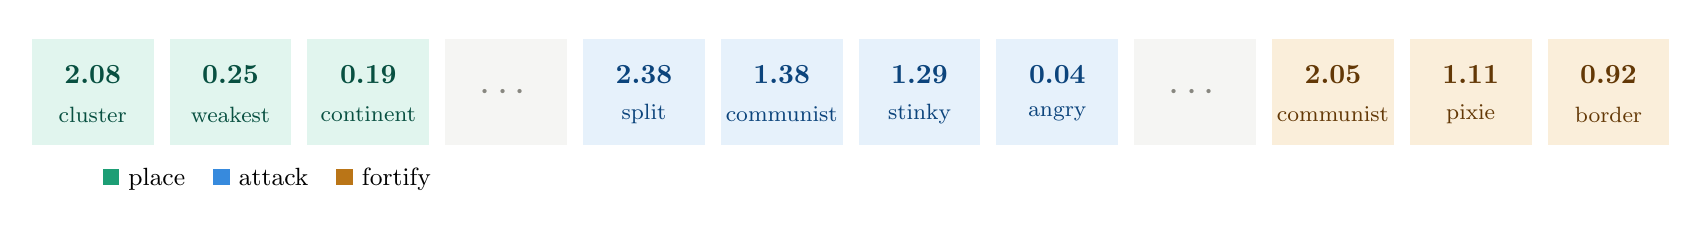
\begin{tikzpicture}[
  cell/.style={
    rectangle,
    minimum width=1.6cm,
    minimum height=1.4cm,
    inner sep=2pt,
    draw=white,
    line width=1.5pt
  },
  val/.style={font=\normalsize\bfseries},
  lbl/.style={font=\footnotesize}
]
 
% --- PLACE cells ---
\foreach \i/\v/\n in {0/2.08/cluster, 1/0.25/weakest, 2/0.19/continent} {
  \node[cell, fill=placebg] at (\i*1.75, 0) {};
  \node[val, text=placetxt] at (\i*1.75,  0.22) {\v};
  \node[lbl, text=placetxt] at (\i*1.75, -0.28) {\n};
}
\node[cell, fill=ellipsisbg] at (3*1.75, 0) {};
\node[text=ellipsistxt, font=\Large] at (3*1.75, 0) {$\cdots$};
 
\draw[white, line width=4pt] (3*1.75+0.9, -0.75) -- (3*1.75+0.9, 0.75);
 
% --- ATTACK cells ---
\foreach \i/\v/\n in {0/2.38/split, 1/1.38/communist, 2/1.29/stinky, 3/0.04/angry} {
  \pgfmathsetmacro{\x}{4*1.75 + \i*1.75}
  \node[cell, fill=attackbg] at (\x, 0) {};
  \node[val, text=attacktxt] at (\x,  0.22) {\v};
  \node[lbl, text=attacktxt] at (\x, -0.28) {\n};
}
\node[cell, fill=ellipsisbg] at (8*1.75, 0) {};
\node[text=ellipsistxt, font=\Large] at (8*1.75, 0) {$\cdots$};
 
\draw[white, line width=4pt] (8*1.75+0.9, -0.75) -- (8*1.75+0.9, 0.75);
 
% --- FORTIFY cells ---
\foreach \i/\v/\n in {0/2.05/communist, 1/1.11/pixie, 2/0.92/border} {
  \pgfmathsetmacro{\x}{9*1.75 + \i*1.75}
  \node[cell, fill=fortifybg] at (\x, 0) {};
  \node[val, text=fortifytxt] at (\x,  0.22) {\v};
  \node[lbl, text=fortifytxt] at (\x, -0.28) {\n};
}
 
% --- Legend ---
\node[right] at (0, -1.1) {%
  \textcolor{placeacc}{\rule{0.6em}{0.6em}}~{\small place}\quad
  \textcolor{attackacc}{\rule{0.6em}{0.6em}}~{\small attack}\quad
  \textcolor{fortifyacc}{\rule{0.6em}{0.6em}}~{\small fortify}
};
 
\end{tikzpicture}
}% end scalebox
\end{center}
\vfill
\end{frame}
	% =============================================================================
	\section{Primi Risultati}
	
	\begin{frame}{\centering Primi Risultati , Setup Sperimentale}
		
		\begin{center}
			\small
			1000 partite a 4 giocatori $\cdot$ mappa standard Risk $\cdot$
			100 turni massimi $\cdot$ seed fisso per riproducibilità
		\end{center} 

		\vspace{0.2cm}
		
		\begin{adjustbox}{width=\textwidth}
			\small
			\renewcommand{\arraystretch}{1.25}
			\begin{tabular}{lcccccc}
				\toprule
				\textbf{Bot} & \textbf{Win\%} & \textbf{Avg Rank} & \textbf{Avg Territories}
				& \textbf{Avg Armies} & \textbf{Survived\%}\\
				\midrule
				Angry  (Aggressivo)  & 9.03\% & 3.39 & 7.22 & 11.61 & 13.22\%  \\
				Stinky (Opportunista)  & 28.42\% & 2.44 & 12.6 & 63.97 & 41.19\% \\
				Communist (Egualitario)& 8.79\% & 3.04 & 3.77 & 154.41 & 18.57\%  \\
				Cluster (Confine) & 19.83\% & 2.42 & 7.27 & 313.81 & 36.7\% \\
				Pixie (Continentale)    & 11.07\% & 2.23 & 5.3 & 242.36 & 39.34\% \\
				\textbf{RLGA} (Evolutivo) & \textbf{54.5\%} & \textbf{1.86} & \textbf{22.64} & \textbf{269.14}
				& \textbf{69.3\%}\\
				\bottomrule
			\end{tabular}
		\end{adjustbox}
		
		\begin{flushleft}
			\tiny Tabella contenente nome bot, percentuale winrate, media posizione in classifica,
			media territori posseduti a fine partita, media armate a fine partita
			percentuale di sopravvivenza nelle 1000 partite.
		\end{flushleft}
		
		\vspace{0.2cm}
		\begin{itemize}
			\item<1-> \textbf{Baseline}: i bot hand-coded forniscono un punto di
			riferimento stabile e riproducibile.
			\item<2-> \textbf{RLGA vs. baseline}: si valuta se l'evoluzione converge
			verso strategie dominanti in un numero ragionevole di generazioni.
		\end{itemize}
	\end{frame}
	
	\begin{frame}{\centering Primi Risultati , Osservazioni Qualitative}
		
		\begin{columns}[T]
			\begin{column}{0.48\textwidth}
				\begin{block}{Comportamenti emergenti}
					\small
					\begin{itemize}
						\item \textbf{Angry} domina nelle fasi iniziali grazie alla pressione
						costante, ma si espone a contrattacchi coordinati per la
						mancanza di difesa passiva.
						\item \textbf{Cluster} costruisce posizioni solide ma tarda ad
						espandersi se il cluster di partenza è piccolo.
						\item \textbf{Communist} regge bene nelle partite lunghe grazie
						all'equalizzazione, ma è lento a conquistare.
						\item \textbf{RLGA} in fase di training mostra rapida convergenza
						nei pesi di attacco, mentre il fortify rimane più variabile.
					\end{itemize}
				\end{block}
			\end{column}
			\begin{column}{0.48\textwidth}
				\vspace{0.1cm}
				\begin{block}{Limitazioni attuali}
					\small
					\begin{itemize}
						\item Il fitness di RLGA è sensibile al \alert{numero di avversari}
						e alla loro composizione.
						\item La \alert{stocasticità} dei dadi rende necessarie molte
						partite per stimare il win-rate in modo affidabile.
						\item Il framework non supporta ancora \alert{mappe personalizzate}
						nel loop di training automatico.
					\end{itemize}
				\end{block}
				\vspace{0.2cm}
				\begin{alertblock}{Prossimo passo}
					\small
					Estendere la batteria di test a \alert{50+ run} per bot e
					aggiungere intervalli di confidenza alle metriche.
				\end{alertblock}
			\end{column}
		\end{columns}
	\end{frame}
	
	% =============================================================================
	\section{Conclusioni}
	
	\begin{frame}{\centering Conclusioni}
		
		\onslide<1->{
			\begin{block}{Framework modulare}
				Un motore di simulazione Risk completo in Python, con
				\alert{separazione netta} tra logica di gioco, bot e agenti intelligenti.
			\end{block}
		}
		\vspace{0.2cm}
		\onslide<2->{
			\begin{block}{Bot di riferimento}
				Cinque strategie hand-coded ispirate alla letteratura (\textit{Angry},
				\textit{Stinky}, \textit{Communist}, \textit{Cluster}, \textit{Pixie})
				coprono uno \alert{spazio strategico ampio} e riproducibile.
			\end{block}
		}
		\vspace{0.2cm}
		\onslide<3->{
			\begin{block}{Agente evolutivo RLGA}
				Il genoma a macro-azioni con \alert{selezione softmax} e operatori
				genetici standard converge verso comportamenti competitivi
				in modo interpretabile.
			\end{block}
		}
		\vspace{0.2cm}
		\onslide<4->{
			\begin{alertblock}{Lavoro futuro}
				\begin{itemize}
					\item Batteria di test \alert{più dettagliata e sistematica}.
					\item \alert{Nuove strategie} note in letteratura per ampliare
					il benchmark e confrontare approcci eterogenei.
					\item \alert{Altri approcci di ML}.
				\end{itemize}
			\end{alertblock}
		}
	\end{frame}
	
	\section{Grazie per l'attenzione}
	
\end{document}